% XeLaTeX can use any Mac OS X font. See the setromanfont command below.
% Input to XeLaTeX is full Unicode, so Unicode characters can be typed directly into the source.

% The next lines tell TeXShop to typeset with xelatex, and to open and save the source with Unicode encoding.

\documentclass[11pt, a4paper, oneside]{article}
\usepackage[spanish]{babel}

%\usepackage[parfill]{parskip}    % Activate to begin paragraphs with an empty line rather than an indent
\usepackage{graphicx}

% Will Robertson's fontspec.sty can be used to simplify font choices.
% To experiment, open /Applications/Font Book to examine the fonts provided on Mac OS X,
% and change "Hoefler Text" to any of these choices.

\usepackage{fontspec,xltxtra,xunicode}
\defaultfontfeatures{Mapping=tex-text}
\setromanfont[Mapping=tex-text]{Book Antiqua}
\setsansfont[Scale=MatchLowercase,Mapping=tex-text]{Gill Sans}
\setmonofont[Scale=0.9]{Courier}

% para el cdigo fuente
\usepackage{listings}
\lstset{
basicstyle=\small\ttfamily,
commentstyle=\itshape\ttfamily,
keywordstyle=\bfseries\ttfamily,
showspaces=false,
showstringspaces=false,
tabsize=2,
extendedchars=true,
language=ruby}

%\renewcommand{\contentsname}{Contenido}
%\renewcommand{\partname}{Parte}
%\renewcommand{\indexname}{Lista Alfabética}
%\renewcommand{\appendixname}{Apéndice}
\renewcommand{\figurename}{Figura}
%\renewcommand{\listfigurename}{Lista de Figuras}
%\renewcommand{\tablename}{Tabla}
%\renewcommand{\listtablename}{Lista de Tablas}
%\renewcommand{\chaptername}{Capítulo}

%\setlength{\epigraphwidth}{180pt}
%\epigraph{Cualquier tecnología lo suficientemente avanzada es indistinguible de la magia.}{Perfiles del Futuro\\\textsc{Arthur C. Clarke}, escritor}

\title{ShowMe}
\author{Ernesto Jiménez}
\date{\today}                                           % Activate to display a given date or no date

\begin{document}
\maketitle

\section{¿Qué es ShowMe?}

\textbf{ShowMe} es una aplicación \emph{mashup} que proporciona servicios orientados al ocio y turismo a usuarios de dispositivos móviles. La idea es que el usuario envíe en un mensaje con su localización actual y qué información quiere obtener, y la aplicación le contesta con un mensaje que contiene un mapa con los sitios que él ha solicitado ya marcados.

Actualmente, ShowMe proporciona los siguientes servicios:

\begin{itemize}
	\item \textbf{Ocio}: busca locales comerciales y de ocio (restaurantes, farmacias, etc).
	\item \textbf{Eventos}: busca eventos que se van a celebrar, o se están celebrando ya, próximamente en el lugar indicado (conciertos, exposiciones, etc.)
	\item \textbf{Turismo}: busca lugares de interés próximos al lugar indicado (monumentos, edificios históricos, playas, etc.)
\end{itemize}

\section{APIs utilizadas}

Listado de las APIs que utiliza ShowMe:

\subsection*{Recepción de SMS (Open Movilforum)}
Esta API permite la recepción de mensajes de texto (SMS), para su posterior proceso. En la aplicación se usa para recibir el \emph{input} del usuario.

\texttt{http://open.movilforum.com/apirecepcion}

\subsection*{Envío HTTP de MMS (Open Movilforum)}
Permite el envío vía web de mensajes multimedia (MMS) a teléfonos móviles. ShowMe la utiliza para enviar la imagen con el mapa y un texto informativo al teléfono móvil del usuario.

\texttt{http://open.movilforum.com/node/205}

\subsection*{Google Maps API}
De la API de Google Maps, se utilizan dos servicios:

\textbf{Geocoding} permite transformar una dirección (por ejemplo, ``Plaza de los Luceros, Alicante'') en coordenadas geográficas (latitud y longitud). ShowMe utiliza este servicio para obtener las coordenadas de la dirección que proporciona el usuario.

\textbf{Static Maps} proporciona imágenes estáticas de mapas creados a partir de coordenadas. ShowMe lo utiliza para obtener el mapa con los resultados que se le enviará al usuario.

\texttt{http://code.google.com/apis/maps/documentation/services.html}\\
\texttt{http://code.google.com/apis/maps/documentation/staticmaps/}

\subsection*{Yahoo! Upcoming API}
\textbf{Yahoo! Upcoming} proporciona información de eventos (conciertos, exposiciones, ferias, evento deportivos, etc) cercanos a una localización concreta. ShowMe emplea esta API para proporcionar el servicio de \texttt{Eventos}.

\texttt{http://upcoming.yahoo.com/services/api/}

\subsection*{Geonames Wikipedia Geocoding}
El servicio web \textbf{Geonames Wikipedia Geocoding} proporciona una lista de artículos geolocalizados de la Wikipedia que se encuentren cerca de la dirección proporcionada. ShowMe lo emplea para el servicio de \texttt{Turismo}.

\texttt{http://www.geonames.org/export/wikipedia-webservice.html}

\subsection{11870 API}

La API de 11870 permite buscar lugares de ocio, locales comerciales y servicios cerca de una determinada dirección. ShowMe la utiliza para proporcionar el servicio de \texttt{Ocio}.

\texttt{http://11870.com/api}

\section{¿Cómo funciona?} % (fold)
\label{sec:_cómo_funciona}

En la figura~\ref{fig:diagrama} se muestra el flujo de procesamiento desde que al sistema le llega un mensaje de un usuario, hasta que le envía un mensaje con el mapa solicitado.

\begin{figure}[htp]
\centering
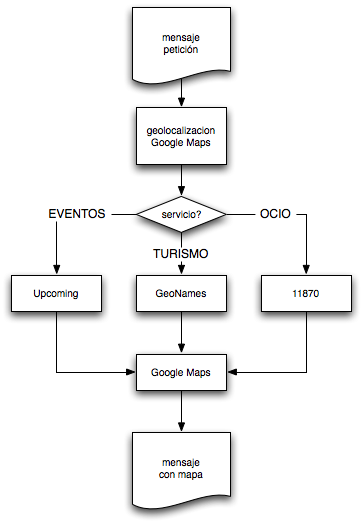
\includegraphics[width=8cm]{showme_diagram.png}
\caption{Flujo de ShowMe}
\label{fig:diagrama}
\end{figure}

El proceso es el siguiente:

\begin{enumerate}
	\item Se recibe un \textbf{mensaje} del usuario (ya sea SMS con la API de \textbf{Recepción de SMS de Open Movilforum} o un e-mail utilizando GMail).
	\item Se \textbf{geolocaliza} (con la API de \textbf{Google Maps}) la dirección postal indicada en el mensaje, para obtener sus coordenadas geográficas.
	\item Se procede una \textbf{búsqueda} para obtener una lista de localizaciones con las que formar el mapa. En función de la palabra clave indicada en el mensaje, se selecciona un servicio u otro:
	\begin{itemize}
		\item \textbf{Ocio}: se llama a la API de \textbf{11870}.
		\item \textbf{Eventos}: se llama a la API de \textbf{Yahoo! Upcoming}.
		\item \textbf{Turismo}: se llama a la API de \textbf{GeoNames}.
	\end{itemize}
	\item Con la lista de localizaciones, se construye un mapa gracias a la API de \textbf{Google Maps}.
	\item Se le envía de vuelta un mensaje al usuario con una imagen adjunta del mapa. Este mensaje puede ser un MMS (API de \textbf{Envío HTTP de MMS de Open Movilforum}) o un e-mail (librería GMail), en función de si el usuario solicitó el servicio mediante SMS o e-mail.
\end{enumerate}

En cuanto a la sintaxis de los SMS enviados por los usuarios, debe ser la siguiente:

\begin{itemize}
	\item \textbf{Ocio}: \texttt{OCIO locales a buscar~: dirección} (ejemplo: \texttt{OCIO restaurantes baratos: plaza de los luceros, alicante}).
	\item \textbf{Eventos}: \texttt{EVENTOS dirección} (ejemplo: \texttt{EVENTOS barcelona})
	\item \textbf{Turismo}: \texttt{TURISMO dirección} (ejemplo: \texttt{TURISMO alicante})
\end{itemize}

% section _cómo_funciona (end)

\section{Ámbitos de aplicación} % (fold)
\label{sec:Ámbitos_de_aplicación}

Con los servicios proporcionados actualmente (\textbf{Ocio}, \textbf{Eventos} y \textbf{Turismo}), ShowMe es útil para:

\begin{itemize}
	\item Habitantes de una ciudad que se encuentren en un apuro en la calle y quieran encontrar una farmacia de guardia, restaurantes cercanos, gasolineras, etc.
	\item Turistas en una ciudad que no conozcan y quieran saber qué sitios pueden visitar, si hay algún evento (exposiciones, conciertos, etc) por la zona, y buscar locales comerciales (supermercados, hoteles, restaurantes, etc). 
\end{itemize}

% section Ámbitos_de_aplicación (end)

\section{Posibles mejoras y ampliaciones} % (fold)
\label{sec:posibles_mejoras_y_ampliaciones}

Una posibilidad interesante para mejorar ShowMe sería la de utilizar la API de \textbf{Localízame}, que proporciona las coordenadas geográficas en las que está el usuario, y así evitaría tener que escribir una dirección postal en el texto del mensaje.

\textbf{ShowMe} está diseñado de forma modular y extensible, se pueden añadir nuevos servicios a los ya existentes de forma sencilla sin que haya que cambiar el código fuente ya escrito.

\section{Detalles de implementación} % (fold)
\label{sec:detalles_de_implementación}

La aplicación está programada con \textbf{Ruby}, por ser un lenguaje orientado a objetos legible y conciso.

\textbf{ShowMe} está dividido en tres grandes módulos:

\begin{itemize}
	\item Recepción de mensajes
	\item Procesamiento
	\item Envío de mensajes
\end{itemize}

\subsection{Sobre la recepción de mensajes}

La \textbf{recepción} de mensajes se realiza mediante la API de recepción de SMSs de Open Movilforum. Esta API nos proporciona un número de móvil que va ligado a una dirección de e-mail a la que se envían los SMS. Por lo tanto, la API nos permite acceder a los SMS como si fuesen e-mails.

La técnica habitual para explotar esta API es monitorizar la cuenta de correo cada cierto tiempo para comprobar si hay mensajes que procesar. ShowMe sin embargo ofrece tres posibilidades para usar esta API:
\begin{itemize}
	\item Monitorizar una cuenta de GMail.
	\item Monitorizar una cuenta de correo mediante POP3.
	\item \textbf{Arrancar en el puerto 25 un pequeño servidor SMTP}.
\end{itemize}

Mientras que las dos primeras soluciones son muy buenas para hacer pruebas, no son una solución robusta de cara a montar servicios en producción. Es debido a esta inconveniencia que ShowMe funciona por defecto arrancando un pequeño servidor SMTP en el puerto 25 que se encarga de recibir los SMS en tiempo real en lugar de examinar una cuenta de correo cada cierto tiempo.

Además, el código dedicado a la recepción de está totalmente desligado de la aplicación ShowMe. Los servicios siguen un \textbf{patrón Observador} pudiendo suscribir cualquier observador al servicio de recogida de mensajes (en nuestro caso el motor de procesamiento de ShowMe).

\subsection{Sobre el procesamiento}

El \textbf{procesamiento} es el núcleo de la aplicación, y es la que se encarga de procesar el mensaje de entrada al sistema, y de generar el mensaje de salida.

Para ello, cada vez que llega un mensaje de entrada, un \textbf{proxy} analiza el texto de mensaje y extrae la palabra clave. En función de la palabra clave, se llama a un servicio con el mismo nombre. Por ejemplo, un mensaje recibido con el texto \texttt{``OCIO restaurantes: plaza luceros alicante''} identificaría la palabra clave \texttt{OCIO} y llamaría a ese servicio.

Todos los servicios tienen un \emph{modus operandi} similar:

\begin{enumerate}
	\item \textbf{Geolocalizan} la dirección
	\item Llaman a la \textbf{API correspondiente}, a la que proporcionan las coordenadas obtenidas anteriormente, y reciben una lista con localizaciones relevantes.
	\item Construyen un \textbf{mapa} con esas localizaciones y la API de Google Maps.
	\item Proporcionan un \textbf{mensaje} al módulo de envío de mensajes.
\end{enumerate}

\subsection{Sobre el envío de mensajes}

Los mensajes con el mapa se pueden enviar tanto por \textbf{e-mail} (utilizando una librería para GMail) como por \textbf{MMS}.

\textbf{NOTA IMPORTANTE:}

Dado que la API para envío HTTP de MMS de Open Movilforum ya no funciona (la web que proporciona el servicio ha cambiado), se ha optado por implementar una \textbf{versión propia} de esa API. Gracias a la librería \texttt{Mechanize} para Ruby, se automatiza el comportamiento de un visitante humano a la web y se realizan las mismas acciones (rellenar campos de formulario, clicks del ratón, etc.) para envíar un MMS con una imagen adjunta.

Sin embargo, dado que la nueva web de Movistar es reciente, parece que a día de hoy \textbf{todavía están haciendo cambios} (incluso el servidor estuvo caído por momentos), así que es posible que falle (en concreto, hace dos días funcionaba y ahora el mismo código en ocasiones da un Error 500).

% section detalles_de_implementación (end)

% section posibles_mejoras_y_ampliaciones (end)
\end{document}
